% This is samplepaper.tex, a sample chapter demonstrating the
% LLNCS macro package for Springer Computer Science proceedings;
% Version 2.21 of 2022/01/12
%
\documentclass[runningheads]{llncs}
\bibliographystyle{splncs04}
\usepackage{algorithm}
\usepackage{algorithmic}
\usepackage{comment}
\usepackage{url}
\usepackage{bm}
\usepackage{multirow}
\usepackage{amsmath}
\usepackage{booktabs}
%\usepackage{multirow}
\usepackage[T1]{fontenc}
% T1 fonts will be used to generate the final print and online PDFs,
% so please use T1 fonts in your manuscript whenever possible.
% Other font encondings may result in incorrect characters.
%
\usepackage{graphicx}
% Used for displaying a sample figure. If possible, figure files should
% be included in EPS format.
%
% If you use the hyperref package, please uncomment the following two lines
% to display URLs in blue roman font according to Springer's eBook style:
%\usepackage{color}
%\renewcommand\UrlFont{\color{blue}\rmfamily}
%\urlstyle{rm}
%
\usepackage{color}

\begin{document}

%
%\title{Neural Architecture Search Model Improvement: a single-objective and  multi-objective study}

\title{Improving Neural Architecture Search Models with Evolutionary Algorithms}


%\title{A Study on Neural Architecture Search Model Improvement with Evolutionary Algorithms}

\titlerunning{Improving Neural Architecture Search Models with Evolutionary Algorithms}

%
%\titlerunning{Abbreviated paper title}
% If the paper title is too long for the running head, you can set
% an abbreviated paper title here
%
\author{ }
%\author{Ruben Café\inst{1} \and
%Nuno Leite\inst{1}\orcidID{0000-0001-6328-3579} \and
%Artur Ferreira\inst{1,2}\orcidID{0000-0002-6508-0932}
%}


%
\authorrunning{ }
%\authorrunning{R. Café et al.}
% First names are abbreviated in the running head.
% If there are more than two authors, 'et al.' is used.
%


\institute{ }
%\institute{ISEL, Instituto Superior de Engenharia de Lisboa, 
%Instituto Polit\'ecnico de Lisboa \and
%IDMEC, IST – Instituto Superior Técnico, Lisboa, PORTUGAL \\
%\email{a42176@alunos.isel.pt} 
%\hspace{.5cm}
%\email{nuno.leite@isel.pt} 
%\hspace{.5cm}
%\email{artur.ferreira@isel.pt} 
%}
%
\maketitle          
%
\begin{abstract}
Neural Architecture Search (NAS) is an adequate technique to automate the design of neural networks suitable for machine learning tasks. However, the quality of the results depend on the search algorithm and on whether efficiency is optimized alongside accuracy. This paper presents a detailed comparison of optimizers for NAS on the tabular NAS-Bench-201 benchmark (CIFAR-10, CIFAR-100, and ImageNet16-120 datasets), under identical budgets and fixed seeds, across two distinct formulations: single-objective and multi-objective. In the single-objective study, we compare four evolutionary algorithms, the Genetic Algorithm (GA), Self-Adaptive Differential Evolution (SADE), Adaptive Inertia Weight Particle Swarm Optimization (AIW-PSO) and the Grey Wolf Optimization (GWO), against Bayesian Optimization (BO). We consider two fitness functions,
driven solely by accuracy or by accuracy against Floating Point Operations (FLOPs). In the multi-objective study, we compare native Pareto optimizers, Non-dominated Sorting Genetic Algorithm II (NSGA-II), Generalized Differential Evolution III (GDE3) and the Bayesian q-Expected Hypervolume Improvement (qEHVI). As the benchmark exposes the exact optimum and Pareto front, the methods are evaluated with the accuracy gap, the hypervolume, and the IGD$^{+}$ indicator, complemented by the search wall-clock and a Wilcoxon signed-rank test. BO and the self-adaptive evolutionary algorithms reach the optimum, but BO's search is several hundred times slower (roughly $450\times$); for multiple objectives, native search dominates scalarization, and GDE3 is the best performing method under this protocol, pairing the smallest gap to the true Pareto front with a per-run cost of a few seconds. %The optimizer should therefore be matched to the problem formulation.

\keywords{
Artificial Intelligence 
\and
Convolutional Neural Networks
\and 
Evolutionary Algorithms 
\and
Machine Learning 
\and
NAS-Bench-201.}
\and
Neural Architecture Search 
\end{abstract} 


%
% 1 - Introduction
%
\section{Introduction}\label{SEC1}
\noindent 
Deep learning models, and Convolutional Neural Networks (CNN)~\cite{lecun1998gradient} in particular, achieve state-of-the-art results across computer-vision tasks. However, their performance depends on the network architecture and on the many design choices that accompany it. As models grow deeper and more sophisticated, the number of these choices grows rapidly and manual design becomes impractical. Neural Architecture Search (NAS) addresses this by turning the topology of the network itself into the object of optimization~\cite{avval2025systematic}, automatically searching a space of candidate architectures for one that maximizes a given target metric.

A NAS method couples a search space with a search strategy and a validation strategy~\cite{avval2025systematic}. The search strategy is decisive: reinforcement learning, differentiable relaxations, Bayesian Optimization (BO)~\cite{snoek2012bo} and Evolutionary Algorithms (EA)~\cite{eiben2015ec} have all been used, and EA are particularly attractive because they are gradient-free and naturally handle the discrete, categorical and mixed-variable spaces that NAS produces. However, most studies introduce a single new method, compare it against a small set of baselines on one benchmark, and report a single run per algorithm. It therefore remains unclear how standard optimizers behave relative to one another under an identical budget and seed protocol, and whether a ranking established on one problem transfers to another.

A second limitation is that accuracy alone is rarely the deployment objective. Practical models must also be efficient in terms of model size, latency or Floating-Point Operations (FLOPs), which turns architecture search into a Multi-Objective Optimization (MOO) problem~\cite{zhao2024lamoo}: instead of a single optimum one seeks the Pareto front of non-dominated trade-offs. Two strategies are common. A single-objective optimizer can be made cost-aware by scalarizing accuracy and cost into a weighted sum and sweeping the weight, or a native multi-objective optimizer such as Non-dominated Sorting Genetic Algorithm II (NSGA-II)~\cite{deb2002nsga2}, Generalized Differential Evolution III (GDE3)~\cite{kukkonen2005gde3} or the Bayesian q-Expected Hypervolume Improvement (qEHVI)~\cite{daulton2020qehvi} can evolve the whole population toward the Pareto front. The preferable strategy, and at what computational cost, is rarely quantified under controlled conditions.

This paper presents a detailed comparison of optimizers for NAS on the NAS-Bench-201 benchmark~\cite{dong2020nasbench201}, using CIFAR-10, CIFAR-100 and ImageNet16-120 under identical budgets and fixed seeds. Because the benchmark is tabular, every architecture is pre-trained and each evaluation reduces to a lookup, so both the global optimum and the exact Pareto front are known by enumeration and can serve as a reference. The study is organized as two complementary case studies. The first treats NAS as a single-objective problem and compares four EA, the Genetic Algorithm (GA)~\cite{goldberg1989genetic}, Self-Adaptive Differential Evolution (SADE)~\cite{qin2009sade}, Adaptive Inertia Weight Particle Swarm Optimization (AIW-PSO)~\cite{qin2006aiwpso} and the Grey Wolf Optimization (GWO)~\cite{mirjalili2014gwo}, against BO, both for maximizing accuracy and for a scalarized accuracy--cost objective. The second treats NAS as a multi-objective problem and compares the native optimizers NSGA-II, GDE3, and qEHVI against that scalarized baseline. The methods are assessed with the accuracy gap to the known optimum, the hypervolume~\cite{zitzler1999hv} and the Inverted Generational Distance Plus (IGD$^{+}$)~\cite{ishibuchi2015igdplus} indicator against the exact front, the search wall-clock, and a Wilcoxon signed-rank test.

The contributions of this paper are four-fold. First, we address a single-objective comparison of five optimizers across three datasets of increasing difficulty, analyzing convergence, distance to the known optimum, reliability across seeds, architectural diversity, and per-algorithm search cost. Second, a direct comparison of native multi-objective search against a scalarized single-objective baseline, evaluated with two complementary indicators, the hypervolume and IGD$^{+}$, and supported by a statistical test. Third, evidence that, under the benchmark, budget and encoding studied here, GDE3 is significantly the best of the multi-objective methods compared, that NSGA-II and qEHVI are statistically indistinguishable, and that native search recovers the high-accuracy region that scalarization systematically misses. Finally, a compute-cost analysis showing that the Gaussian-process methods (BO and qEHVI) are orders of magnitude slower than the evolutionary alternatives, so that the choice of optimizer should be matched to the problem formulation and budget rather than to a fixed ranking.

The remainder of this paper is organized as follows. Section~\ref{SEC2} reviews the relevant background and related work. Section~\ref{SEC3} describes the proposed approach. Section~\ref{SEC4} reports and discusses the experimental evaluation, and Section~\ref{SEC5} presents the conclusions and directions for future work.


%%%%%%%%%%%%%%%%%%%%%%%%%%%%%%%%%%%%%%%%%%%%%%%%%%%%%%%%%%%
% Section 2
%%%%%%%%%%%%%%%%%%%%%%%%%%%%%%%%%%%%%%%%%%%%%%%%%%%%%%%%%%%

\section{Related Work} \label{SEC2}
\noindent This section introduces NAS and its components (Section~\ref{SEC2.1}), evolutionary algorithms for NAS (Section~\ref{SEC2.2}), and multi-objective optimization for architecture search (Section~\ref{SEC2.3}).

%
% 2.1 - Neural Architecture Search
%
\subsection{Neural Architecture Search} \label{SEC2.1}
A NAS method is commonly decomposed into search space, search strategy, and validation strategy~\cite{avval2025systematic}. CNN remain dominant for spatial data~\cite{lecun1998gradient,younesi2024convolutions}, and the growing number of design choices motivates automation within AutoML~\cite{he2019automl}. Cell-based search spaces, introduced with normal and reduction cells~\cite{zoph2018nasnet}, dominate by retaining expressive connectivity while drastically shrinking the space. Among search strategies, reinforcement learning first surpassed hand-designed models but at prohibitive cost; EA match or surpass it at comparable or lower cost~\cite{avval2025systematic}, while differentiable relaxations such as DARTS~\cite{liu2019darts} have lower complexity, but may be unstable and suffer from a discretization gap. The validation strategy dominates the cost, motivating weight-sharing supernets~\cite{cai2020ofa}, one-shot, and training-free estimators~\cite{mellor2021nwot}. Tabular benchmarks such as NAS-Bench-201~\cite{dong2020nasbench201} and NATS-Bench~\cite{dong2021natsbench}, and hardware-aware variants like HW-NAS-Bench~\cite{li2021hwnasbench}, pre-compute every architecture's performance in a fixed cell space, decoupling the search strategy from training noise and making the global optimum known by construction; this is essential for the 
comparison study purposes pursued in this paper.


%
% 2.2 - Evolutionary Algorithms for NAS
%
\subsection{Evolutionary Algorithms for NAS} \label{SEC2.2}
EA evolve a population through selection, crossover, and mutation, needing only a fitness value per individual~\cite{eiben2015ec}, which makes them applicable to non-differentiable, mixed-variable, and multi-objective problems~\cite{jiao2024multiobjective}; their use in the Machine Learning (ML) field is known as Evolutionary Machine Learning~\cite{alsahaf2019eml,telikani2021eml}. Architecture search was pioneered by 
Neuro Evolution of Augmenting Topologies (NEAT)~\cite{stanley2002neat}, and regularized (aging) evolution later matched reinforcement learning at equal cost to produce state-of-the-art classifiers~\cite{real2019amoebanet}. Swarm- and differential-evolution-based metaheuristics have also been applied to model configuration~\cite{mohakud2020survey,raiaan2024hpo}, and recent surveys consolidate evolutionary deep learning~\cite{li2022evodl,zhou2021survey}. Some of these works propose a new method against few baselines on a single benchmark; we instead fix a representative set of optimizers and vary the problem formulation, from single- to multi-objective, to isolate how the formulation affects their relative behavior under an identical budget and seed protocol.



%
% 2.3 - Multi-Objective Optimization for NAS
%
\subsection{Multi-Objective Optimization for NAS} \label{SEC2.3}
Deploying a model requires trading accuracy against efficiency metrics such as model size, latency and FLOPs, turning NAS into a Multi-Objective Optimization (MOO) problem~\cite{zhao2024lamoo} whose goal is the Pareto front and the set of non-dominated solutions. Scalarization reduces MOO to a single objective, for instance a weighted sum whose weights are swept to trace the front, but the result is sensitive to the weighting and to the front geometry. Pareto-based evolutionary algorithms instead evolve the whole population toward the front: NSGA-II combines fast non-dominated sorting with a crowding-distance operator~\cite{deb2002nsga2}, and GDE3 extends differential evolution through a one-to-one Pareto selection and the same diversity-preserving truncation~\cite{kukkonen2005gde3}; NSGA-Net applies NSGA-II directly to architecture search~\cite{lu2019nsganet}. On the Bayesian side, qEHVI maximizes the expected hypervolume improvement of a Gaussian-process surrogate~\cite{daulton2020qehvi}. The hypervolume indicator~\cite{zitzler1999hv} is the most common quality measure, as it jointly rewards convergence and diversity without the true front. Recent work accelerates MOO-NAS by partitioning the search space~\cite{zhao2024lamoo} or preserving diversity through novelty search with training-free metrics~\cite{vo2024pdns}.



%%%%%%%%%%%%%%%%%%%%%%%%%%%%%%%%%%%%%%%%%%%%%%%%%%%%%%%%%%%
% Section 3
%%%%%%%%%%%%%%%%%%%%%%%%%%%%%%%%%%%%%%%%%%%%%%%%%%%%%%%%%%%

\section{Proposed Approach} \label{SEC3}
\noindent Section~\ref{SEC3.1} presents the NAS-Bench-201 search space and encoding shared by both case studies. Sections~\ref{SEC3.2} and~\ref{SEC3.3} describe Case Study~1 (single-objective) and Case Study~2 (multi-objective), respectively.

%
% 3.1 - Search Space and Encoding
%
\subsection{Search Space and Encoding for Both Studies} \label{SEC3.1}
Both case studies operate on the cell-based search space of NAS-Bench-201. A candidate is a cell modeled as a directed acyclic graph with four nodes and six edges, where each edge applies one of the five primitive operations listed in Table~\ref{tab:space}. A candidate is encoded as an integer vector of length six over the domain $\{0,\dots,4\}$, yielding $5^6 = 15{,}625$ unique cell topologies. The full network is built by stacking copies of the chosen cell separated by fixed reduction layers; this macro skeleton is not exposed to the optimizer. Since the space is tabular, each candidate is decoded into the corresponding architecture string and the benchmark is queried for its metrics; thus, no network is trained during the search, and both the global accuracy optimum and the exact Pareto front can be obtained by exhaustive enumeration and used as references.

\begin{table}[t]
\centering
\caption{NAS-Bench-201 search space shared by both case studies. The cardinality is $5^6 = 15{,}625$ unique cell topologies.}
\label{tab:space}
\begin{tabular}{cll}
\toprule
\textbf{Index} & \hspace{5mm} \textbf{Operation} & \hspace{5mm}  \textbf{Description} \\
\midrule
0 & \hspace{5mm} \texttt{none}           & \hspace{5mm}  zeroize input \\
1 & \hspace{5mm} \texttt{skip\_connect}  & \hspace{5mm}  identity \\
2 & \hspace{5mm} \texttt{nor\_conv\_1x1} & \hspace{5mm}  $1\times1$ conv + BN + ReLU \\
3 & \hspace{5mm} \texttt{nor\_conv\_3x3} & \hspace{5mm}  $3\times3$ conv + BN + ReLU \\
4 & \hspace{5mm} \texttt{avg\_pool\_3x3} & \hspace{5mm}  $3\times3$ average pooling \\
\bottomrule
\end{tabular}
\end{table}

%
% 3.2 - Case Study 1: Single-Objective NAS
%
\subsection{Case Study 1: Single-Objective NAS} \label{SEC3.2}
This case study treats architecture search as a single-objective problem under two formulations that share the same optimizers. In the first, the goal is to maximize test accuracy, i.e.\ to minimize the fitness function 
given by
  
\begin{equation}
\mathrm{fit}(\mathbf{x}) = 1 - \mathrm{acc}_{\mathrm{test}}(\mathbf{x}),
\label{eq:fit}
\end{equation}

where $\mathrm{acc}_{\mathrm{test}}$ is the benchmark accuracy of the decoded architecture after $200$ epochs of training. The second formulation makes the search cost-aware while keeping it single-objective, by scalarizing accuracy and \#FLOPs into one weighted sum. The cost is the architecture FLOPs normalized to $[0,1]$ over the benchmark,
\begin{equation}
\widehat{\mathrm{FLOPs}}(\mathbf{x}) = \frac{\mathrm{FLOPs}(\mathbf{x}) - \mathrm{FLOPs}_{\min}}{\mathrm{FLOPs}_{\max} - \mathrm{FLOPs}_{\min}},
\label{eq:flops}
\end{equation}
so the two criteria to minimize are
\begin{equation}
f_1(\bm{x}) = 1 - \mathrm{acc}_{\mathbf{test}}(\mathbf{x}), \qquad f_2(\mathbf{x}) = \widehat{\mathrm{FLOPs}}(\mathbf{x}),
\label{eq:objectives}
\end{equation}
and, for a fixed weight $\alpha$, the optimizer minimizes
\begin{equation}
g_\alpha(\mathbf{x}) = \alpha\, f_1(\mathbf{x}) + (1-\alpha)\, f_2(\mathbf{x}).
\label{eq:scalar}
\end{equation}
A larger $\alpha$ favours accuracy and a smaller one favours cost; sweeping $\alpha$ over $\{0.1,0.2,\dots,0.9,1.0\}$ yields ten independent runs per optimizer, whose non-dominated best architectures approximate the accuracy--cost trade-off and serve as the single-objective baseline for Case Study~2.

Five optimizers are used in both formulations. GA~\cite{goldberg1989genetic} evolves fixed-length encodings through selection, crossover, and mutation; SADE~\cite{qin2009sade} adapts its scaling factor, crossover rate and mutation strategy from past trials; AIW-PSO~\cite{qin2006aiwpso} extends PSO~\cite{kennedy1995pso} by drawing each particle toward its personal and the global best with an inertia weight assigned per particle from its fitness rank in the swarm; GWO~\cite{mirjalili2014gwo} mimics the grey-wolf hierarchy and exposes no hyperparameters; and BO~\cite{snoek2012bo}, the non-evolutionary baseline, fits a probabilistic surrogate and maximizes an acquisition function without re-evaluating points. Table~\ref{tab:hyper} reports the configuration used for each of them.

%
% 3.3 - Case Study 2: Multi-Objective NAS
%
\subsection{Case Study 2: Multi-Objective NAS} \label{SEC3.3}
The second case study optimizes the two criteria of Eq.~\eqref{eq:objectives} simultaneously rather than collapsing them into a weighted sum. A solution $\mathbf{x}$ dominates $\mathbf{y}$, written $\mathbf{x} \prec \mathbf{y}$, when it is no worse in both objectives and strictly better in at least one,
\begin{equation}
\mathbf{x} \prec \mathbf{y} \iff f_i(\mathbf{x}) \le f_i(\mathbf{y})\ \ \forall i \in \{1,2\} \ \ \wedge\ \ \exists\, j \in \{1,2\}: f_j(\mathbf{x}) < f_j(\mathbf{y}),
\label{eq:dominance}
\end{equation}
and the goal is to approximate the Pareto front, the set of non-dominated architectures. The quality of an approximation $S$ is measured by its hypervolume, the area of objective space dominated by $S$ and bounded by a reference point $R = (1.1, 1.1)$ placed beyond the worst attainable values~\cite{zitzler1999hv},
\begin{equation}
\mathrm{HV}(S) = \Lambda\!\left( \bigcup_{\bm{x}\in S} \big[f_1(\bm{x}), R_1\big] \times \big[f_2(\bm{x}), R_2\big] \right),
\label{eq:hv}
\end{equation}
where $\Lambda$ denotes the Lebesgue measure~\cite{folland1999real}. Since the benchmark is tabular, the exact Pareto front of each dataset is obtained by enumeration and yields the maximum attainable hypervolume $\mathrm{HV}^{\star}$, so the gap $\mathrm{HV}^{\star}-\mathrm{HV}$ measures how far an algorithm is from the optimum.

Three native multi-objective optimizers are evaluated. The NSGA-II~\cite{deb2002nsga2} and GDE3~\cite{kukkonen2005gde3} approaches evolve a population toward the front and return a single non-dominated set per run, NSGA-II through fast non-dominated sorting with a crowding-distance operator and GDE3 through a one-to-one Pareto selection on a differential-evolution population. The Bayesian method qEHVI~\cite{daulton2020qehvi} fits a Gaussian-process surrogate and proposes, at each step, the architecture expected to enlarge the dominated hypervolume the most. The single-objective optimizers of Case Study~1 act directly on the six integer variables, whereas the three native multi-objective solvers relax them to a continuous domain and round to the nearest operation on evaluation, a standard practice for integer NAS spaces that keeps NSGA-II, GDE3 and qEHVI directly comparable to one another. Table~\ref{tab:hyper} reports the encoding and the hyperparameters of every optimizer of both case studies.


%%%%%%%%%%%%%%%%%%%%%%%%%%%%%%%%%%%%%%%%%%%%%%%%%%%%%%%%%%%
% Section 4
%%%%%%%%%%%%%%%%%%%%%%%%%%%%%%%%%%%%%%%%%%%%%%%%%%%%%%%%%%%
\section{Experimental Evaluation} \label{SEC4}
\noindent Section~\ref{SEC4.1} describes the datasets and protocol followed in the experiments.  Sections~\ref{SEC4.2} and~\ref{SEC4.3} present the single- and multi-objective case studies, respectively. Section~\ref{SEC4.4} provides a discussion about the results.

%
% 4.1 - Datasets and Protocol
%
\subsection{Datasets and Protocol} \label{SEC4.1}
Both case studies use the three datasets bundled with NAS-Bench-201, described in Table~\ref{tab:datasets}: CIFAR-10, CIFAR-100, and the downsampled ImageNet16-120, which provide increasing levels of difficulty. All runs were executed on a machine with the specifications summarized in Table~\ref{tab:machine}. 

Since NAS-Bench-201 is tabular, each evaluation is a benchmark lookup; we therefore distinguish the tabulated training cost of the queried architectures from the search wall-clock, that is, the optimizer's own overhead, and report the latter per algorithm in Case Study~1. The protocol is identical across algorithms within each formulation. In the accuracy-only formulation of Case Study~1, each (algorithm, dataset) pair is run $N_{val}=5$ times with seeds $0$ to $4$ under a budget of $1020$ queries, organized as $20$ initial individuals plus $50$ generations of $20$ offspring, or for BO as $20$ random startup trials plus $1000$ guided trials. In the scalarized formulation of Case Study~1, the same budget is spent once per weight $\alpha\in\{0.1,0.2,\dots,0.9,1.0\}$, and each configuration is repeated over $N_{val}=3$ seeds. Including $\alpha=1$ lets the sweep optimize accuracy with no cost penalty at all, so the high-accuracy endpoint of the front is reachable in principle. The assembled scalarized front therefore consumes ten times the per-run budget of a native multi-objective search ($10 \times 1020$ versus $1020$ evaluations), so the comparison in Case Study~2 is generous to scalarization. In Case Study~2, each native optimizer (NSGA-II, GDE3, and qEHVI) is run with $N_{val}=3$ independent seeds under the same $1020$-evaluation budget. For every setting, we report the aggregated convergence behavior, the distribution of the final result across repetitions, and condensed summary statistics.

Table~\ref{tab:hyper} reports the configuration of every optimizer. The hyperparameters follow the values recommended in the original publications, or the defaults of the corresponding library when the publication leaves them open, and they were held fixed across the three datasets, the nine $\alpha$ weights and all seeds. In particular, the surrogate and the acquisition function of the two Gaussian-process methods (BO and qEHVI) were not re-tuned per dataset. No method therefore benefits from dataset-specific tuning, which keeps the comparison budget-matched and free of tuning bias; the counterpart is that a per-dataset tuned version of any of these optimizers could outperform the results reported here.

\begin{table}[!ht]
\centering
\caption{Configuration of every optimizer. All runs evolve a population (or swarm) of $20$ individuals over $50$ generations, for a total of $1020$ evaluations; the two Gaussian-process methods spend the same budget as startup plus guided trials. An integer encoding operates directly on the six edge variables in $\{0,\dots,4\}$, whereas a real encoding relaxes them to a continuous domain and rounds to the nearest operation on evaluation. In both cases the variables are box-constrained to the operation range, the bounded variation operators of each library keep offspring inside it, and any residual out-of-range value is repaired by rounding and clamping to $\{0,\dots,4\}$ before the benchmark is queried, so no candidate is ever discarded as infeasible. The values are identical for the three datasets, for the nine $\alpha$ weights of the scalarized formulation, and for all seeds.}
\label{tab:hyper}
\small
\setlength{\tabcolsep}{4pt}
\begin{tabular}{@{}llp{7.2cm}@{}}
\toprule
\textbf{Algorithm} & \textbf{Encoding} & \textbf{Hyperparameters} \\
\midrule
\multicolumn{3}{@{}l}{\textit{\textbf{Case Study 1 (single-objective)}}} \\
GA      & integer       & $p_c = 0.9$ (uniform crossover), $p_m = 0.05$ (multi-point bit-flip), tournament selection with $k = 20\%$ of the population \\
SADE    & integer       & none: $F$, $CR$ and the mutation strategy are self-adapted from the success history of past trials \\
AIW-PSO & integer       & $c_1 = c_2 = 2.05$; the inertia weight $w$ is assigned per particle from its fitness rank in the swarm, with adaptation amplitude $\alpha_w = 0.4$ (unrelated to the scalarization weight $\alpha$) \\
GWO     & integer       & none: the coefficients $a$, $A$ and $C$ are derived from the iteration counter \\
BO      & integer       & Gaussian-process surrogate; Expected Improvement acquisition with $\xi = 0.01$; $20$ random startup trials $+$ $1000$ guided trials \\
\midrule
\multicolumn{3}{@{}l}{\textit{\textbf{Case Study 2 (multi-objective, native)}}} \\
NSGA-II & real, rounded & SBX crossover ($p_c = 0.9$, $\eta_c = 15$) and polynomial mutation ($p_m = 1/6$, $\eta_m = 20$) \\
GDE3    & real, rounded & DE/rand/1/bin with $F = 0.5$ and $CR = 0.9$ \\
qEHVI   & real, rounded & Gaussian-process surrogate with standardized outputs; batch size $q = 5$, $128$ Monte-Carlo samples, $10$ restarts and $128$ raw samples for the acquisition optimization; $20$ Sobol startup points $+$ $200$ batches \\
\bottomrule
\end{tabular}
\end{table}

\begin{table}[t]
\centering
\caption{Datasets used in this work, all bundled with NAS-Bench-201.}
\label{tab:datasets}
\begin{tabular}{lcc}
\toprule
\textbf{Dataset} & \hspace{5mm} \textbf{Classes} & \hspace{5mm} \textbf{Input shape} \\
\midrule
CIFAR-10       & \hspace{5mm} 10  & \hspace{5mm} $32\times32\times3$ \\
CIFAR-100      & \hspace{5mm} 100 & \hspace{5mm} $32\times32\times3$ \\
ImageNet16-120 & \hspace{5mm} 120 & \hspace{5mm} $16\times16\times3$ \\
\bottomrule
\end{tabular}
\end{table}


\begin{table}[t]
\centering
\caption{Hardware and software environment used to run the experiments.}
\label{tab:machine}
\begin{tabular}{ll}
\toprule
\textbf{Component} & \textbf{Specification} \\
\midrule
CPU              & \textit{AMD Ryzen 7 7700X 8-Core Processor} \\
RAM              & \textit{32.0 GB} \\
GPU              & \textit{NVIDIA GeForce RTX 5060 Ti} \\
Operating system & \textit{Ubuntu 22.04 LTS} \\
Python version   & \textit{3.11} \\
Key libraries    & pymoo \textit{0.6.1.6}, BoTorch \textit{0.16.1}, NAS-Bench-201 API \textit{1.8} \\
\bottomrule
\end{tabular}
\end{table}


%
% 4.2 - Case Study 1: Single-Objective NAS
%
\subsection{Case Study 1: Single-Objective NAS} \label{SEC4.2}
Since the optimum solution for each dataset is known by exhaustive enumeration, Figure~\ref{fig:nas_gap} tracks the gap between the running best test accuracy and the corresponding optimum on a logarithmic scale, such that exposes differences that a linear axis would miss. On CIFAR-10 and CIFAR-100 datasets, every method except AIW-PSO essentially reaches the upper bound; GA is the fastest to descend but plateaus marginally short on CIFAR-10, while SADE, GWO and BO close the gap entirely on both. On ImageNet16-120 dataset, the methods separate with BO driving the gap to machine-precision zero, SADE and GWO descending roughly two further orders of magnitude after generation 15, GA plateauing around $10^{-4}$ on CIFAR-10 and around $5 \times 10^{-3}$ on ImageNet16-120, and AIW-PSO never descending below roughly $2 \times 10^{-3}$. The exhaustive upper bounds on test accuracy are $0.9437$, $0.7351$ and $0.4731$ on CIFAR-10, CIFAR-100, and ImageNet16-120, respectively. Table~\ref{tab:cs1arch} consolidates the final accuracy of each algorithm along with the cost (\#FLOPs and parameters) of the selected architecture: on CIFAR-10 and CIFAR-100 the methods that reach the upper bound converge to the same architecture, whereas AIW-PSO settles on less
computationally intensive, but less accurate cells.

\begin{figure}[ht]
\centering
\includegraphics[width=\textwidth]{figs/cs1_gap_grid.pdf}
\vspace{-4mm}
\caption{NAS-Bench-201 distance to the exhaustive upper bound over generations (mean over five seeds). The floor at $10^{-6}$ signals convergence to the optimum (lower is better).}
\label{fig:nas_gap}
\end{figure}

\begin{table}[!ht]
\centering
\caption{Case Study 1 (accuracy-only formulation): mean final test accuracy and the cost (\#FLOPs, \#Params) of the best architecture selected by each algorithm ($\pm$ std over $N_{val}=5$ seeds); a zero std is omitted. Accuracies matching the exhaustive upper bound (given in the text) are in boldface.}
\label{tab:cs1arch}
\setlength{\tabcolsep}{3pt}
\resizebox{\textwidth}{!}{%
\begin{tabular}{lccccccccc}
\toprule
& \multicolumn{3}{c}{\textbf{CIFAR-10}} & \multicolumn{3}{c}{\textbf{CIFAR-100}} & \multicolumn{3}{c}{\textbf{ImageNet16-120}} \\
\cmidrule(lr){2-4} \cmidrule(lr){5-7} \cmidrule(lr){8-10}
\textbf{Algorithm} & \textbf{Acc.} & \textbf{\#FLOPs} & \textbf{\#Par.} & \textbf{Acc.} & \textbf{\#FLOPs} & \textbf{\#Par.} & \textbf{Acc.} & \textbf{\#FLOPs} & \textbf{\#Par.} \\
\midrule
GA      & $0.9436{\pm}.0003$ & $140.7{\pm}28.1$ & $0.99{\pm}.19$ & $\bm{0.7351}$ & $184.7$ & $1.29$ & $0.4686{\pm}.0041$ & $27.7{\pm}4.3$ & $0.79{\pm}.12$ \\
SADE    & $\bm{0.9437}$ & $153.3$ & $1.07$ & $\bm{0.7351}$ & $184.7$ & $1.29$ & $0.4719{\pm}.0027$ & $32.0{\pm}3.5$ & $0.91{\pm}.10$ \\
AIW-PSO & $0.9417{\pm}.0028$ & $165.9{\pm}30.4$ & $1.16{\pm}.21$ & $0.7327{\pm}.0036$ & $158.8{\pm}35.6$ & $1.12{\pm}.24$ & $0.4674{\pm}.0047$ & $33.2{\pm}4.7$ & $0.94{\pm}.13$ \\
GWO     & $\bm{0.9437}$ & $153.3$ & $1.07$ & $\bm{0.7351}$ & $184.7$ & $1.29$ & $0.4722{\pm}.0021$ & $31.8{\pm}3.1$ & $0.90{\pm}.08$ \\
BO      & $\bm{0.9437}$ & $153.3$ & $1.07$ & $\bm{0.7351}$ & $184.7$ & $1.29$ & $\bm{0.4731}$ & $30.5$ & $0.87$ \\
\bottomrule
\end{tabular}}
\end{table}

Reliability across the five seeds confirms this picture. On the two easier datasets only AIW-PSO is unstable, whereas on ImageNet16-120 the methods separate, with BO placing every run at the optimum, GWO and SADE within $10^{-3}$ of it, and GA and AIW-PSO showing the largest spreads and the lowest medians; the corresponding standard deviations are reported in Table~\ref{tab:cs1arch}.

Architectural diversity, measured as the mean number of distinct cells visited per run out of the 15{,}625 possibilities, is governed by the algorithm rather than by the dataset: about $120$ unique cells for GA, $300$ for SADE, $400$ for GWO, $500$ for AIW-PSO, and the full $1020$ queries without repetition for BO. Each algorithm stays within the same band on the three datasets, all differences being within one standard deviation.

The optimizers also differ sharply in search cost. Since the benchmark is tabular, a run's wall-clock reflects optimizer overhead rather than network training: the evolutionary algorithms complete a $1020$-evaluation run in about $6$~seconds, whereas BO requires roughly $2700$~seconds, as reported in Table~\ref{tab:time}, about $450\times$ more, due to its Gaussian-process surrogate that scales cubically with the number of evaluations. The tabulated training cost of the queried architectures, by contrast, is comparable across methods, so BO reaches the optimum but at a search cost two orders of magnitude above the evolutionary algorithms.

\begin{table}[!ht]
\centering
\caption{Mean search wall-clock per run (elapsed seconds) for the three formulations. As the benchmark is tabular, this is optimizer overhead, not network training. All three blocks use the same encoding for every optimizer (Table~
ef{tab:hyper}); in particular the Bayesian optimizer declares the six edges as integer variables in both single-objective formulations, so the two BO rows are directly comparable. The Gaussian-process methods (BO and qEHVI) scale cubically with the number of evaluations, which is what separates them from the evolutionary algorithms}
\label{tab:time}
\begin{tabular}{lccc}
\toprule
\textbf{Algorithm} & \hspace{5mm} \textbf{CIFAR-10} & \hspace{5mm}  \textbf{CIFAR-100} & \hspace{5mm}  \textbf{ImageNet16-120} \\
\midrule
\multicolumn{4}{l}{\textit{\textbf{Case Study 1 (single-objective, accuracy only)}}} \\
GA      & \hspace{5mm} $5.9$ & \hspace{5mm} $6.3$ & \hspace{5mm} $6.0$ \\
SADE    & \hspace{5mm} $5.6$ & \hspace{5mm} $6.4$ & \hspace{5mm} $6.2$ \\
AIW-PSO & \hspace{5mm} $8.4$ & \hspace{5mm} $6.4$ & \hspace{5mm} $6.9$ \\
GWO     & \hspace{5mm} $7.5$ & \hspace{5mm} $6.2$ & \hspace{5mm} $6.2$ \\
BO      & \hspace{5mm} $2716.3$ & \hspace{5mm} $2747.7$ & \hspace{5mm} $2697.1$ \\
\midrule
\multicolumn{4}{l}{\textit{\textbf{Case Study 1 (single-objective, accuracy--\#FLOPs; per $\alpha$ run)}}} \\
GA      & \hspace{5mm} $13.4$ & \hspace{5mm} $6.8$ & \hspace{5mm} $6.4$ \\
SADE    & \hspace{5mm} $6.2$ & \hspace{5mm} $3.8$ & \hspace{5mm} $4.2$ \\
AIW-PSO & \hspace{5mm} $7.0$ & \hspace{5mm} $5.2$ & \hspace{5mm} $4.8$ \\
GWO     & \hspace{5mm} $4.1$ & \hspace{5mm} $3.7$ & \hspace{5mm} $3.4$ \\
BO      & \hspace{5mm} $901.4$ & \hspace{5mm} $889.9$ & \hspace{5mm} $985.7$ \\
\midrule
\multicolumn{4}{l}{\textit{\textbf{Case Study 2 (multi-objective, native)}}} \\
NSGA-II & \hspace{5mm} $11.5$ & \hspace{5mm} $12.1$ & \hspace{5mm} $10.9$ \\
GDE3    & \hspace{5mm} $25.4$ & \hspace{5mm} $19.3$ & \hspace{5mm} $18.0$ \\
qEHVI   & \hspace{5mm} $3269.9$ & \hspace{5mm} $2480.5$ & \hspace{5mm} $2211.5$ \\
\bottomrule
\end{tabular}
\end{table}

Beyond maximizing accuracy alone, the same optimizers were applied to the scalarized accuracy--cost objective of Eq.~\eqref{eq:scalar}, which keeps the search single-objective while making it cost-aware. Figure~\ref{fig:cs1_scalar_fronts} shows, for each optimizer, the non-dominated set assembled from its ten $\alpha$ runs overlaid on the exact front. The sweep now includes $\alpha=1$, which places no weight at all on cost, so the high-accuracy endpoint is targeted directly rather than merely approached. Even so, every scalarized front stays measurably inside the exact front, and the residual gap is therefore a property of the weighted-sum aggregation itself, not of where the sweep was truncated. 

\begin{figure}[!ht]
\centering
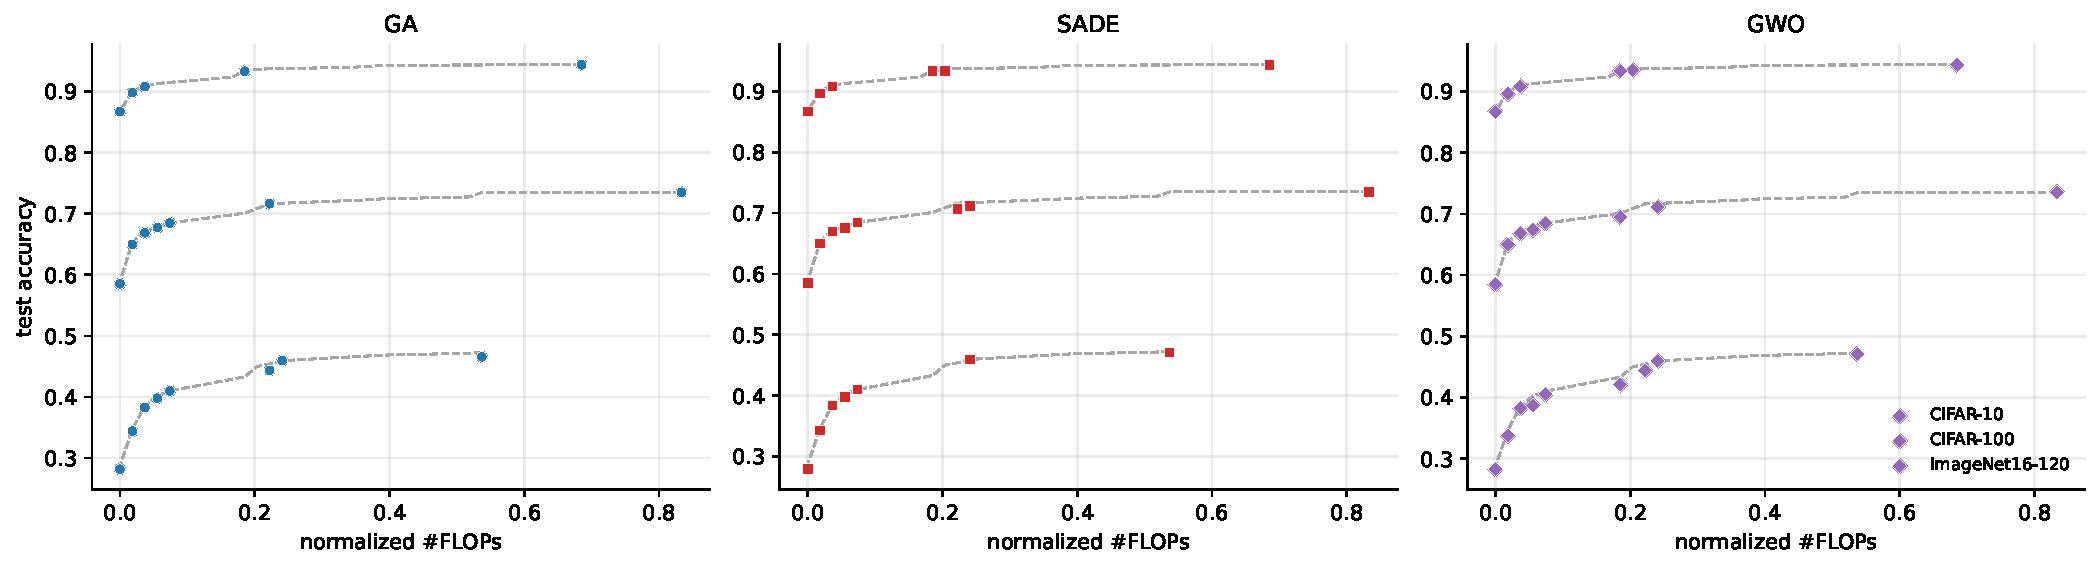
\includegraphics[width=\textwidth]{figs/cs1_scalar_fronts_a.pdf}\\[2mm]
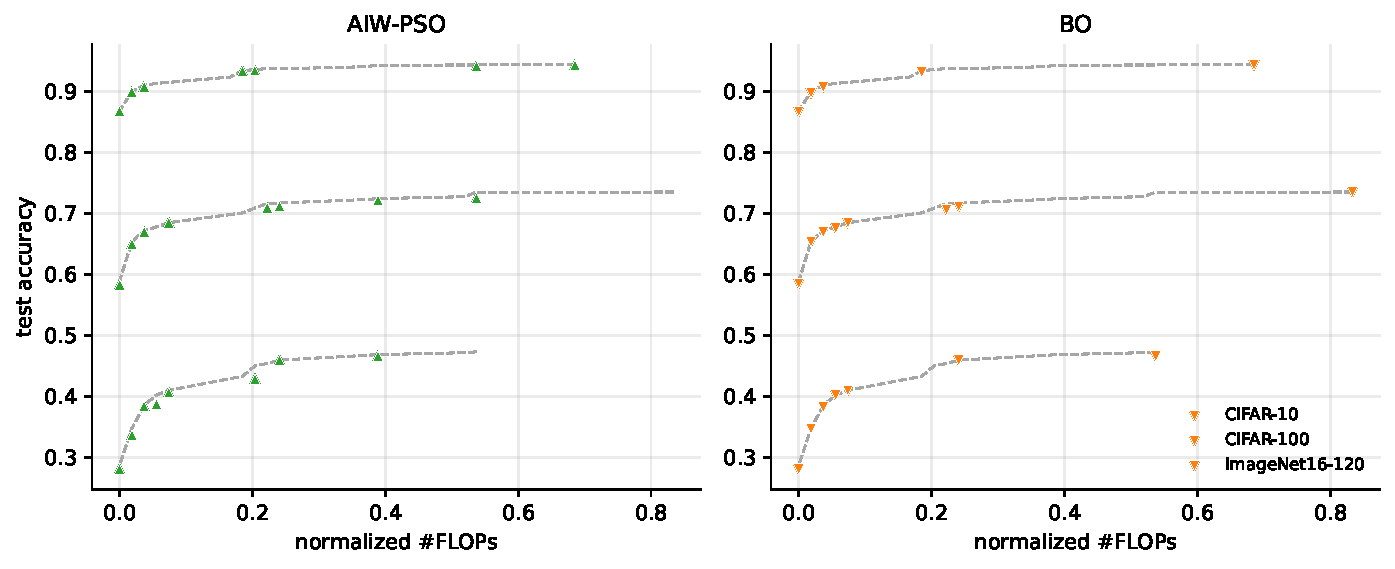
\includegraphics[width=\textwidth]{figs/cs1_scalar_fronts_b.pdf}
\caption{Case Study 1, scalarized formulation: non-dominated set assembled by each optimizer from its nine $\alpha$ runs, shown per optimizer and overlaid on the exact front (dashed); each panel contains the three datasets, which occupy distinct accuracy bands. All optimizers concentrate in the low-cost region and stop short of the high-accuracy end of the front.}
\label{fig:cs1_scalar_fronts}
\end{figure}

Figure~\ref{fig:alpha_sweep} plots the accuracy--\#FLOPs trajectory as $\alpha$ is swept from $0.1$ to $0.9$, and Table~\ref{tab:alpha_sweep} documents the exact architecture returned at representative $\alpha$ values (top-1 accuracy, \#FLOPs, and \#Params); the five trajectories almost coincide, indicating that the scalarized optimizers explore essentially the same trade-off and differ mainly in how far they push along it. Table~\ref{tab:cs1_scalar_hv} summarizes the quality of these assembled fronts as their hypervolume and gap to $\mathrm{HV}^{\star}$; the values are close to one another and, as Case Study~2 shows, below those reached by native multi-objective search.

\begin{figure}[!ht]
\centering												  
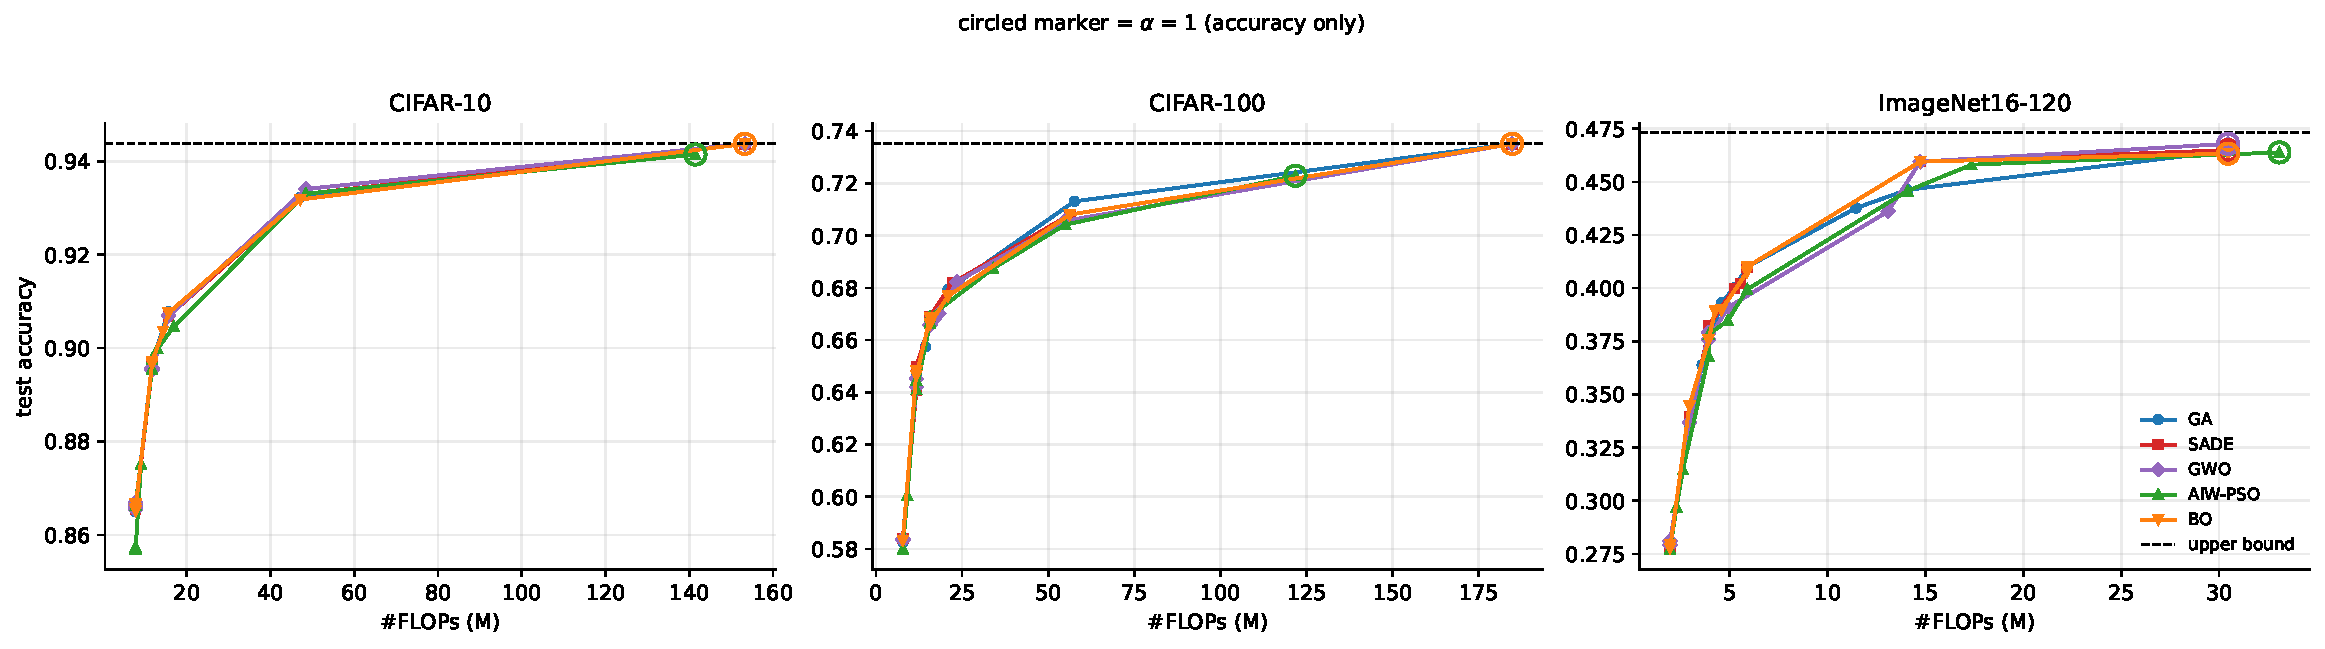
\includegraphics[width=\textwidth]{figs/cs2_alpha_sweep.pdf}
\caption{Scalarization $\alpha$-sweep: accuracy versus \#FLOPs of the architecture found by each scalarized algorithm as the weight $\alpha$ is swept from $0.1$ (cost-oriented) to $0.9$ (accuracy-oriented), per dataset. The five trajectories almost coincide, showing that the scalarized optimizers trace essentially the same accuracy--cost front.}
\label{fig:alpha_sweep}
\end{figure}

\begin{table}[!ht]
\centering
\caption{Scalarization $\alpha$-sweep: architecture returned by each scalarized algorithm at representative weights $\alpha \in \{0.1, 0.3, 0.5, 0.7, 0.9, 1.0\}$, reported as Top-1 accuracy\,/\,\#FLOPs~(M)\,/\,\#Params~(M) (mean over 3 seeds). Larger $\alpha$ favours accuracy, smaller $\alpha$ favours cost. Figure~\ref{fig:alpha_sweep} shows the complete sweep over the nine weights.}
\label{tab:alpha_sweep}
\setlength{\tabcolsep}{3pt}
\resizebox{\textwidth}{!}{%
\begin{tabular}{clccccc}
\toprule
\textbf{Dataset} & $\mathbf{\alpha}$ & \textbf{GA} & \textbf{SADE} & \textbf{GWO} & \textbf{AIW-PSO} & \textbf{BO} \\
\midrule
\multirow{6}{*}{CIFAR-10} & 0.1 & 0.865\,/\,7.8\,/\,0.07 & 0.867\,/\,7.8\,/\,0.07 & 0.865\,/\,7.8\,/\,0.07 & 0.857\,/\,7.8\,/\,0.07 & 0.867\,/\,7.8\,/\,0.07 \\
 & 0.3 & 0.867\,/\,7.8\,/\,0.07 & 0.866\,/\,7.8\,/\,0.07 & 0.866\,/\,7.8\,/\,0.07 & 0.875\,/\,9.1\,/\,-- & 0.865\,/\,7.8\,/\,0.07 \\
 & 0.5 & 0.897\,/\,11.7\,/\,0.10 & 0.896\,/\,11.7\,/\,0.10 & 0.896\,/\,11.7\,/\,0.10 & 0.896\,/\,11.7\,/\,0.10 & 0.897\,/\,11.7\,/\,0.10 \\
 & 0.7 & 0.908\,/\,15.6\,/\,0.13 & 0.907\,/\,15.6\,/\,0.13 & 0.907\,/\,15.6\,/\,0.13 & 0.900\,/\,13.0\,/\,-- & 0.904\,/\,14.3\,/\,-- \\
 & 0.9 & 0.932\,/\,47.1\,/\,0.34 & 0.933\,/\,48.4\,/\,-- & 0.934\,/\,48.4\,/\,-- & 0.933\,/\,48.4\,/\,-- & 0.932\,/\,47.1\,/\,0.34 \\
 & 1 & 0.944\,/\,153.3\,/\,1.07 & 0.944\,/\,153.3\,/\,1.07 & 0.944\,/\,153.3\,/\,1.07 & 0.941\,/\,141.5\,/\,-- & 0.944\,/\,153.3\,/\,1.07 \\
\midrule
\multirow{6}{*}{CIFAR-100} & 0.1 & 0.583\,/\,7.8\,/\,0.08 & 0.584\,/\,7.8\,/\,0.08 & 0.583\,/\,7.8\,/\,0.08 & 0.580\,/\,7.8\,/\,0.08 & 0.583\,/\,7.8\,/\,0.08 \\
 & 0.3 & 0.647\,/\,11.7\,/\,0.11 & 0.641\,/\,11.7\,/\,0.11 & 0.642\,/\,11.7\,/\,0.11 & 0.644\,/\,11.7\,/\,0.11 & 0.648\,/\,11.7\,/\,0.11 \\
 & 0.5 & 0.657\,/\,14.3\,/\,-- & 0.667\,/\,15.7\,/\,0.14 & 0.666\,/\,15.7\,/\,0.14 & 0.666\,/\,15.7\,/\,0.14 & 0.668\,/\,15.7\,/\,0.14 \\
 & 0.7 & 0.671\,/\,18.3\,/\,-- & 0.669\,/\,15.7\,/\,0.14 & 0.670\,/\,18.3\,/\,-- & 0.669\,/\,15.7\,/\,0.14 & 0.666\,/\,15.7\,/\,0.14 \\
 & 0.9 & 0.713\,/\,57.6\,/\,-- & 0.708\,/\,56.3\,/\,-- & 0.706\,/\,55.0\,/\,0.41 & 0.704\,/\,55.0\,/\,0.41 & 0.708\,/\,56.3\,/\,-- \\
 & 1 & 0.735\,/\,184.7\,/\,1.29 & 0.735\,/\,184.7\,/\,1.29 & 0.735\,/\,184.7\,/\,1.29 & 0.723\,/\,121.8\,/\,0.86 & 0.735\,/\,184.7\,/\,1.29 \\
\midrule
\multirow{6}{*}{ImageNet16-120} & 0.1 & 0.279\,/\,2.0\,/\,0.08 & 0.278\,/\,2.0\,/\,0.08 & 0.279\,/\,2.0\,/\,0.08 & 0.277\,/\,2.0\,/\,0.08 & 0.279\,/\,2.0\,/\,0.08 \\
 & 0.3 & 0.336\,/\,2.9\,/\,0.11 & 0.339\,/\,2.9\,/\,0.11 & 0.337\,/\,2.9\,/\,0.11 & 0.315\,/\,2.6\,/\,-- & 0.344\,/\,2.9\,/\,0.11 \\
 & 0.5 & 0.393\,/\,4.6\,/\,-- & 0.382\,/\,3.9\,/\,0.14 & 0.379\,/\,3.9\,/\,0.14 & 0.378\,/\,3.9\,/\,0.14 & 0.389\,/\,4.2\,/\,-- \\
 & 0.7 & 0.410\,/\,5.9\,/\,0.19 & 0.402\,/\,5.6\,/\,-- & 0.391\,/\,4.9\,/\,0.16 & 0.399\,/\,5.9\,/\,0.19 & 0.408\,/\,5.9\,/\,0.19 \\
 & 0.9 & 0.446\,/\,14.1\,/\,-- & 0.460\,/\,14.7\,/\,0.44 & 0.460\,/\,14.7\,/\,0.44 & 0.458\,/\,17.4\,/\,-- & 0.460\,/\,14.7\,/\,0.44 \\
 & 1 & 0.465\,/\,30.5\,/\,0.87 & 0.465\,/\,30.5\,/\,0.87 & 0.468\,/\,30.5\,/\,0.87 & 0.464\,/\,33.1\,/\,-- & 0.463\,/\,30.5\,/\,0.87 \\
\bottomrule
\end{tabular}}
\end{table}

\begin{table}[!ht]
\centering
\caption{Case Study 1, scalarized formulation: mean hypervolume $\pm$ std over $N_{val}=3$ seeds of the front assembled from the ten $\alpha$ runs, with the gap to the true Pareto front $(\mathrm{HV}^{\star}-\mathrm{HV})$ in parentheses; the reference point is $R=(1.1,1.1)$. The true-front hypervolume $\mathrm{HV}^{\star}$ is in the last row.}
\label{tab:cs1_scalar_hv}   
\resizebox{\textwidth}{!}{%
\begin{tabular}{lccc}
\toprule
\textbf{Algorithm} & \textbf{CIFAR-10} & \textbf{CIFAR-100} & \textbf{ImageNet16-120} \\
\midrule
GA      & $1.1348 \pm 0.0004$ $(5.4{\times}10^{-3})$ & $0.8898 \pm 0.0019$ $(1.1{\times}10^{-2})$ & $0.6002 \pm 0.0017$ $(1.0{\times}10^{-2})$ \\
SADE    & $1.1350 \pm 0.0004$ $(5.2{\times}10^{-3})$ & $0.8872 \pm 0.0020$ $(1.4{\times}10^{-2})$ & $0.6020 \pm 0.0029$ $(8.7{\times}10^{-3})$ \\
GWO     & $1.1354 \pm 0.0003$ $(4.7{\times}10^{-3})$ & $0.8857 \pm 0.0049$ $(1.5{\times}10^{-2})$ & $0.6015 \pm 0.0045$ $(9.1{\times}10^{-3})$ \\
AIW-PSO & $1.1342 \pm 0.0011$ $(5.9{\times}10^{-3})$ & $0.8864 \pm 0.0018$ $(1.4{\times}10^{-2})$ & $0.5993 \pm 0.0025$ $(1.1{\times}10^{-2})$ \\
BO      & $1.1345 \pm 0.0001$ $(5.6{\times}10^{-3})$ & $0.8864 \pm 0.0008$ $(1.4{\times}10^{-2})$ & $0.6013 \pm 0.0014$ $(9.4{\times}10^{-3})$ \\
\midrule
True Pareto front $\mathrm{HV}^{\star}$ & $1.1401$ & $0.9008$ & $0.6107$ \\
\bottomrule
\end{tabular}}
\end{table}



%
% 4.3 - Case Study 2: Multi-Objective NAS
%
\subsection{Case Study 2: Multi-Objective NAS} \label{SEC4.3}
Table~\ref{tab:cs2} reports the hypervolume of the three native optimizers against the exact Pareto front, whose hypervolume $\mathrm{HV}^{\star}$ is $1.1401$, $0.9008$, and $0.6107$ on CIFAR-10, CIFAR-100, and ImageNet16-120, respectively. No single native method dominates: GDE3 attains the highest hypervolume on CIFAR-10 ($1.1382$, a gap of $1.9{\times}10^{-3}$) while NSGA-II leads on CIFAR-100 and ImageNet16-120, and a Wilcoxon signed-rank test~\cite{demsar2006statistical} over the nine (dataset, seed) configurations separates none of the three pairs (GDE3 versus NSGA-II, $p = 1.0$ with GDE3 ahead in five of nine cells; both against qEHVI, $p = 0.20$). Under the coverage-sensitive IGD$^{+}$ indicator (Table~\ref{tab:igd}) the ordering is equally close, with GDE3 best on CIFAR-10 and CIFAR-100 and NSGA-II best on ImageNet16-120. The three native optimizers should therefore be read as equivalent at this budget, with qEHVI consistently last by a small margin and far more expensive.

The separation that does survive is between native search and scalarization, and it is now unambiguous. Every native optimizer attains a higher hypervolume and a lower IGD$^{+}$ than every scalarized one on all three datasets, and the same Wilcoxon test finds the difference significant in $14$ of the $15$ native--scalarized pairs (the exception is qEHVI against SADE, $p = 0.055$). This holds even though the scalarized fronts now include $\alpha=1$ and consume ten times the budget of a single native run, so it can no longer be attributed to a truncated weight sweep: it is the convex-hull limitation of the weighted sum, which cannot recover the concave stretches of the front at any weight.

Figure~\ref{fig:cs2_fronts} shows the Pareto front of each native optimizer in a separate panel, overlaid on the true front (three datasets per panel, in distinct accuracy bands); the optimizers track the entire accuracy--cost curve, so moving down a front cedes a small amount of accuracy for a large reduction in \#FLOPs. Figure~\ref{fig:cs2_conv} reports the hypervolume as a function of the number of evaluations: all three methods converge close to the true-front level, with GDE3 both the highest and the most stable. Table~\ref{tab:mo_tradeoff} makes this trade-off concrete along the best front obtained: on CIFAR-10, conceding about one accuracy point (from $0.9437$ to $0.9336$) already cuts the cost to $31\%$ of the most accurate model, a $0.91$-accuracy architecture needs only $13\%$ of its \#FLOPs, and $0.87$ needs $5\%$; the same pattern holds on CIFAR-100 and ImageNet16-120. The last column shows that NSGA-II and GDE3 recover the whole frontier, including the most accurate architecture, whereas qEHVI matches it everywhere except the top rows. As with BO in Case Study~1, qEHVI carries the overhead of its Gaussian-process surrogate: its runs took on the order of $2700$ seconds, against under $15$ seconds for NSGA-II and GDE3 (Table~\ref{tab:time}), more than two orders of magnitude more, whereas the two evolutionary methods add negligible cost per evaluation.

\begin{table}[!ht]
\centering
\caption{Case Study 2 (multi-objective NAS): mean hypervolume $\pm$ std over $N_{val}=3$ seeds for the three native optimizers, with the gap to the true Pareto front $(\mathrm{HV}^{\star}-\mathrm{HV})$ in parentheses; the reference point is $R=(1.1,1.1)$. Higher hypervolume (and smaller gap) is better. The best value per dataset is in bold. The scalarized single-objective baseline is reported in Table~\ref{tab:cs1_scalar_hv}.}
\label{tab:cs2}
\resizebox{\textwidth}{!}{%
\begin{tabular}{lccc}
\toprule
\textbf{Algorithm} & \textbf{CIFAR-10} & \textbf{CIFAR-100} & \textbf{ImageNet16-120} \\
\midrule
NSGA-II & $1.1365 \pm 0.0009$ $(3.7{\times}10^{-3})$ & $\mathbf{0.8940 \pm 0.0020}$ $(6.8{\times}10^{-3})$ & $\mathbf{0.6061 \pm 0.0010}$ $(4.6{\times}10^{-3})$ \\
GDE3    & $\mathbf{1.1382 \pm 0.0010}$ $(1.9{\times}10^{-3})$ & $0.8934 \pm 0.0020$ $(7.4{\times}10^{-3})$ & $0.6054 \pm 0.0013$ $(5.3{\times}10^{-3})$ \\
qEHVI   & $1.1360 \pm 0.0020$ $(4.1{\times}10^{-3})$ & $0.8928 \pm 0.0030$ $(8.0{\times}10^{-3})$ & $0.6033 \pm 0.0026$ $(7.4{\times}10^{-3})$ \\
\midrule
True Pareto front $\mathrm{HV}^{\star}$ & $1.1401$ & $0.9008$ & $0.6107$ \\
\bottomrule
\end{tabular}}
\end{table}

\begin{table}[!ht]
\centering
\caption{Case Study 2: mean IGD$^{+}$ ($\times 10^{-3}$) $\pm$ std over $N_{val}=3$ seeds to the exact Pareto front (lower is better), for the three native optimizers and the scalarized single-objective baseline of Case Study~1. The best (lowest) value per dataset is in bold. Unlike hypervolume, IGD$^{+}$ explicitly penalizes incomplete coverage of the true front.}
\label{tab:igd}
\setlength{\tabcolsep}{4pt}
\resizebox{\textwidth}{!}{%
\begin{tabular}{lcccccccc}
\toprule
& \multicolumn{3}{c}{\textbf{Native}} & \multicolumn{5}{c}{\textbf{Scalarized}} \\
\cmidrule(lr){2-4} \cmidrule(lr){5-9}
\textbf{Dataset} & \textbf{NSGA-II} & \textbf{GDE3} & \textbf{qEHVI} & \textbf{GA} & \textbf{SADE} & \textbf{GWO} & \textbf{AIW-PSO} & \textbf{BO} \\
\midrule
CIFAR-10       & $3.6{\pm}0.8$ & $\bm{2.2{\pm}0.8}$ & $3.3{\pm}0.8$ & $5.7{\pm}0.5$ & $5.7{\pm}0.5$ & $5.3{\pm}0.3$ & $6.2{\pm}1.2$ & $6.0{\pm}0.1$ \\
CIFAR-100      & $5.7{\pm}1.1$ & $\bm{5.5{\pm}1.3}$ & $5.9{\pm}1.5$ & $10.6{\pm}2.2$ & $11.5{\pm}0.7$ & $13.1{\pm}2.4$ & $13.2{\pm}0.3$ & $12.5{\pm}1.4$ \\
ImageNet16-120 & $\bm{5.3{\pm}0.8}$ & $6.2{\pm}1.3$ & $8.0{\pm}2.0$ & $11.9{\pm}2.2$ & $11.3{\pm}0.7$ & $11.9{\pm}1.5$ & $13.9{\pm}2.2$ & $10.4{\pm}1.1$ \\
\bottomrule
\end{tabular}}
\end{table}

\begin{figure}[ht]
\centering		  
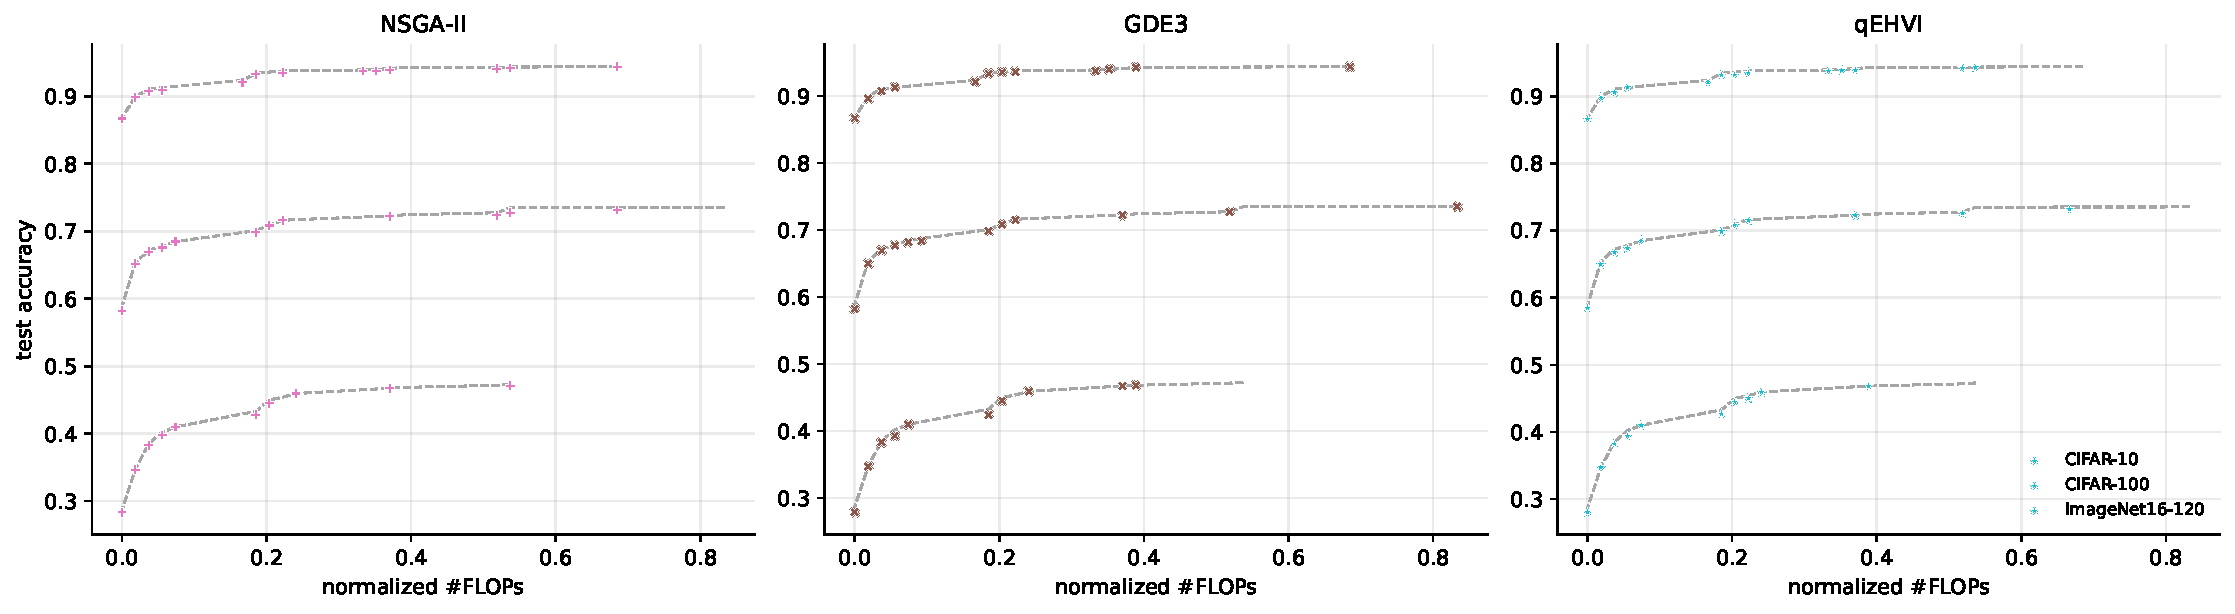
\includegraphics[width=\textwidth]{figs/cs2_fronts_nat.pdf}
\caption{Case Study 2: Pareto front of each native optimizer shown in a separate panel and overlaid on the exact front (dashed); each panel contains the three datasets, which occupy distinct accuracy bands. NSGA-II and GDE3 follow the true front across its full extent, while qEHVI tracks it except at the most accurate, high-FLOPs end.}
\label{fig:cs2_fronts}
\end{figure}

\begin{figure}[ht]
\centering
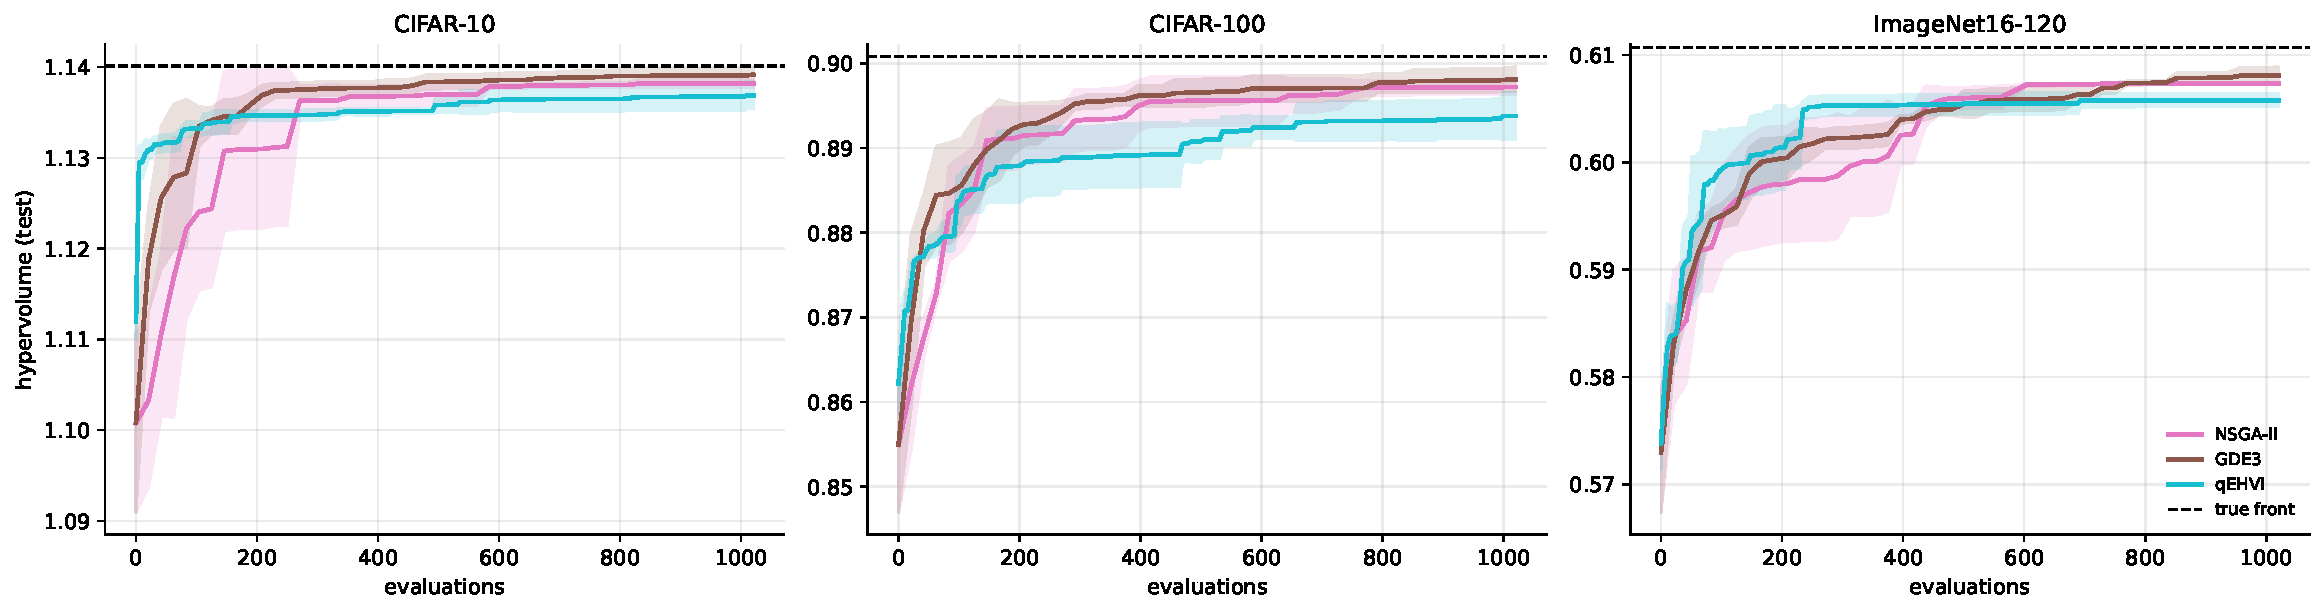
\includegraphics[width=\textwidth]{figs/cs2_hv_convergence_native.pdf}
\caption{Case Study 2: hypervolume versus the number of evaluations, per dataset, for the three native optimizers (mean $\pm$ std over seeds). The dashed line is the true-front hypervolume (higher is better).}		  
\label{fig:cs2_conv}
\end{figure}

\begin{table}[!ht]
\centering
\caption{Accuracy--cost trade-off along the best Pareto front obtained for multi-objective NAS (union of the NSGA-II, GDE3, and qEHVI fronts, aggregated over the three seeds), at representative points per dataset. \#FLOPs (\% of top) is relative to the most accurate architecture. The last column lists which methods recover each accuracy level (N: NSGA-II, G: GDE3, Q: qEHVI).}
\label{tab:mo_tradeoff}
\setlength{\tabcolsep}{5pt}
\scalebox{0.85}{
\begin{tabular}{lccccc}
\toprule
\textbf{Dataset} & \textbf{Top-1 acc.} & \textbf{\#FLOPs (M)} & \textbf{\#Params (M)} & \textbf{\#FLOPs (\%)}  & \textbf{Reached by} \\
\midrule
\multirow{6}{*}{CIFAR-10} & 0.9437 & 153.3 & 1.073 & 100\% & GN \\
 & 0.9402 & 82.5 & 0.587 & 54\% & G \\
 & 0.9363 & 55.0 & 0.400 & 36\% & G \\
 & 0.9213 & 43.2 & 0.316 & 28\% & Gq \\
 & 0.9076 & 15.6 & 0.129 & 10\% & GN \\
 & 0.8672 & 7.8 & 0.073 & 5\% & N \\
\midrule
\multirow{6}{*}{CIFAR-100} & 0.7351 & 184.7 & 1.294 & 100\% & G \\
 & 0.7275 & 121.8 & 0.864 & 66\% & N \\
 & 0.7224 & 86.4 & 0.621 & 47\% & GNq \\
 & 0.6986 & 47.1 & 0.350 & 26\% & GNq \\
 & 0.6773 & 19.6 & 0.163 & 11\% & G \\
 & 0.5852 & 7.8 & 0.079 & 4\% & q \\
\midrule
\multirow{6}{*}{ImageNet16-120} & 0.4708 & 30.5 & 0.866 & 100\% & N \\
 & 0.4673 & 21.6 & 0.623 & 71\% & GN \\
 & 0.4505 & 13.7 & 0.407 & 45\% & q \\
 & 0.4100 & 5.9 & 0.193 & 19\% & GNq \\
 & 0.3833 & 3.9 & 0.137 & 13\% & G \\
 & 0.2837 & 2.0 & 0.081 & 6\% & N \\
\bottomrule
\end{tabular}
}
\end{table}

%
% 4.4 - Discussion
%
\subsection{Discussion of the Experimental Results} \label{SEC4.4}
The two case studies expose complementary behaviors. In the accuracy-only formulation of Case Study~1, benchmark difficulty drives the discrimination among optimizers: on the easier datasets almost every method reaches the optimum, whereas ImageNet16-120 separates them, with BO reaching the bound, SADE and GWO approaching it, GA converging prematurely, and AIW-PSO exploring widely but exploiting poorly. When the same optimizers are made cost-aware through scalarization, they trace nearly identical fronts that stay biased toward the low-cost region and never reach the high-accuracy architectures; this is partly intrinsic to a weighted sum, which cannot recover non-convex portions of a front, and a consequence of capping $\alpha$ at $0.9$, which leaves a residual weight that always rewards cost. 

Case Study~2 shows that handling the two objectives natively removes this bias. On hypervolume, the separation is clearer for GDE3, which is the best method (Wilcoxon, $p \approx 4{\times}10^{-3}$), while NSGA-II and qEHVI are indistinguishable from each other and, on CIFAR-10, even from the scalarized fronts. The coverage-sensitive IGD$^{+}$ indicator resolves this ambiguity (Table~\ref{tab:igd}): every native optimizer dominates every scalarized one on all datasets, because the natives reach the high-accuracy extreme that scalarization omits. GDE3 is the strongest method overall, pairing the smallest gap with the lowest variance across seeds. Notably, it outperforms NSGA-II although both apply the same crowding-distance truncation, which points to the differential-evolution variation operator, rather than diversity preservation alone, as the differentiator. This ranking is established on one tabular benchmark, at a fixed budget of $1020$ evaluations, under a continuous relaxation of a six-variable categorical space, and with one implementation of each optimizer; it should be read as evidence about this setting rather than as a general ordering of multi-objective optimizers for NAS, since larger or hierarchical search spaces, tighter budgets, and noisy (non-tabular) evaluations are all known to change the relative standing of population-based and surrogate-based methods. Reliability therefore deserves to be treated as a primary criterion in both formulations, since averages alone may hide large dispersion and variance, as the GA and AIW-PSO results illustrate. 

Finally, SADE adapts its own control parameters and GWO exposes none, so both ran without any configuration step while remaining competitive in the accuracy-only study. This is a practical advantage in exactly the settings where automated search is needed. Search cost reinforces this reading: the Gaussian-process methods reach strong results but are far more expensive, with BO and qEHVI running more than two orders of magnitude slower per run than the evolutionary algorithms (Table~\ref{tab:time}), so when wall-clock matters the evolutionary methods are preferable.

%
% 5
%
\section{Conclusions} \label{SEC5}
\noindent 
In this paper, we compared evolutionary optimization against Bayesian optimization for NAS on NAS-Bench-201 through two case studies. In single-objective NAS, BO reached the known optimum on each dataset and the self-adaptive SADE and parameter-free GWO matched it on the CIFAR datasets (within $10^{-3}$ on ImageNet16-120), while GA converged prematurely and AIW-PSO was the least reliable; benchmark difficulty drove the discrimination, with only ImageNet16-120 separating the methods. Making the optimizers cost-aware through scalarization produced fronts biased toward low cost that never reached the high-accuracy region. In multi-objective NAS, native search was superior: GDE3 was significantly the best on both hypervolume and IGD$^{+}$ (Wilcoxon, $p \approx 4{\times}10^{-3}$), while NSGA-II and qEHVI were indistinguishable, and every native optimizer dominated every scalarized one under IGD$^{+}$. The Gaussian-process methods (BO and qEHVI) reached strong results but ran more than two orders of magnitude slower per run (Table~\ref{tab:time}), making GDE3 the most attractive of the methods compared here, as it pairs the best fronts with a per-run cost of a few seconds. These conclusions hold for NAS-Bench-201 at a budget of $1020$ evaluations with the encodings and implementations of Table~\ref{tab:hyper}; establishing whether the same ordering survives on larger search spaces, tighter budgets or non-tabular evaluations remains open. The optimizer should be matched to the problem formulation.

As future work, we intend to further explore these techniques with other datasets and to 
consider other multi-objective fitness functions.




\bibliography{bibliography}
\end{document}
